\documentclass[1p]{elsarticle_modified}
%\bibliographystyle{elsarticle-num}

%\usepackage[colorlinks]{hyperref}
%\usepackage{abbrmath_seonhwa} %\Abb, \Ascr, \Acal ,\Abf, \Afrak
\usepackage{amsfonts}
\usepackage{amssymb}
\usepackage{amsmath}
\usepackage{amsthm}
\usepackage{scalefnt}
\usepackage{amsbsy}
\usepackage{kotex}
\usepackage{caption}
\usepackage{subfig}
\usepackage{color}
\usepackage{graphicx}
\usepackage{xcolor} %% white, black, red, green, blue, cyan, magenta, yellow
\usepackage{float}
\usepackage{setspace}
\usepackage{hyperref}

\usepackage{tikz}
\usetikzlibrary{arrows}

\usepackage{multirow}
\usepackage{array} % fixed length table
\usepackage{hhline}

%%%%%%%%%%%%%%%%%%%%%
\makeatletter
\renewcommand*\env@matrix[1][\arraystretch]{%
	\edef\arraystretch{#1}%
	\hskip -\arraycolsep
	\let\@ifnextchar\new@ifnextchar
	\array{*\c@MaxMatrixCols c}}
\makeatother %https://tex.stackexchange.com/questions/14071/how-can-i-increase-the-line-spacing-in-a-matrix
%%%%%%%%%%%%%%%

\usepackage[normalem]{ulem}

\newcommand{\msout}[1]{\ifmmode\text{\sout{\ensuremath{#1}}}\else\sout{#1}\fi}
%SOURCE: \msout is \stkout macro in https://tex.stackexchange.com/questions/20609/strikeout-in-math-mode

\newcommand{\cancel}[1]{
	\ifmmode
	{\color{red}\msout{#1}}
	\else
	{\color{red}\sout{#1}}
	\fi
}

\newcommand{\add}[1]{
	{\color{blue}\uwave{#1}}
}

\newcommand{\replace}[2]{
	\ifmmode
	{\color{red}\msout{#1}}{\color{blue}\uwave{#2}}
	\else
	{\color{red}\sout{#1}}{\color{blue}\uwave{#2}}
	\fi
}

\newcommand{\Sol}{\mathcal{S}} %segment
\newcommand{\D}{D} %diagram
\newcommand{\A}{\mathcal{A}} %arc


%%%%%%%%%%%%%%%%%%%%%%%%%%%%%5 test

\def\sl{\operatorname{\textup{SL}}(2,\Cbb)}
\def\psl{\operatorname{\textup{PSL}}(2,\Cbb)}
\def\quan{\mkern 1mu \triangleright \mkern 1mu}

\theoremstyle{definition}
\newtheorem{thm}{Theorem}[section]
\newtheorem{prop}[thm]{Proposition}
\newtheorem{lem}[thm]{Lemma}
\newtheorem{ques}[thm]{Question}
\newtheorem{cor}[thm]{Corollary}
\newtheorem{defn}[thm]{Definition}
\newtheorem{exam}[thm]{Example}
\newtheorem{rmk}[thm]{Remark}
\newtheorem{alg}[thm]{Algorithm}

\newcommand{\I}{\sqrt{-1}}
\begin{document}

%\begin{frontmatter}
%
%\title{Boundary parabolic representations of knots up to 8 crossings}
%
%%% Group authors per affiliation:
%\author{Yunhi Cho} 
%\address{Department of Mathematics, University of Seoul, Seoul, Korea}
%\ead{yhcho@uos.ac.kr}
%
%
%\author{Seonhwa Kim} %\fnref{s_kim}}
%\address{Center for Geometry and Physics, Institute for Basic Science, Pohang, 37673, Korea}
%\ead{ryeona17@ibs.re.kr}
%
%\author{Hyuk Kim}
%\address{Department of Mathematical Sciences, Seoul National University, Seoul 08826, Korea}
%\ead{hyukkim@snu.ac.kr}
%
%\author{Seokbeom Yoon}
%\address{Department of Mathematical Sciences, Seoul National University, Seoul, 08826,  Korea}
%\ead{sbyoon15@snu.ac.kr}
%
%\begin{abstract}
%We find all boundary parabolic representation of knots up to 8 crossings.
%
%\end{abstract}
%\begin{keyword}
%    \MSC[2010] 57M25 
%\end{keyword}
%
%\end{frontmatter}

%\linenumbers
%\tableofcontents
%
\newcommand\colored[1]{\textcolor{white}{\rule[-0.35ex]{0.8em}{1.4ex}}\kern-0.8em\color{red} #1}%
%\newcommand\colored[1]{\textcolor{white}{ #1}\kern-2.17ex	\textcolor{white}{ #1}\kern-1.81ex	\textcolor{white}{ #1}\kern-2.15ex\color{red}#1	}

{\Large $\underline{11a_{135}~(K11a_{135})}$}

\setlength{\tabcolsep}{10pt}
\renewcommand{\arraystretch}{1.6}
\vspace{1cm}\begin{tabular}{m{100pt}>{\centering\arraybackslash}m{274pt}}
\multirow{5}{120pt}{
	\centering
	\includegraphics[width=112pt]{../../../GIT/diagram.site/Diagrams/png/384_11a_135.png}\\
\ \ \ A knot diagram\footnotemark}&
\allowdisplaybreaks
\textbf{Linearized knot diagam} \\
\cline{2-2}
 &
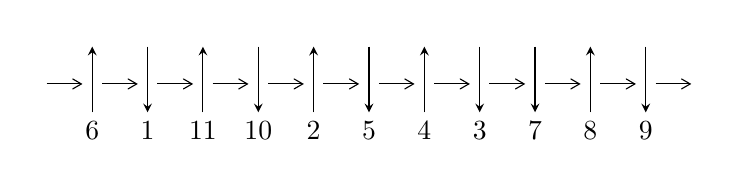
\begin{tikzpicture}[x=20pt, y=17pt]
	% nodes
	\node (C0) at (0, 0) {};
	\node (C1) at (1, 0) {};
	\node (C1U) at (1, +1) {};
	\node (C1D) at (1, -1) {6};

	\node (C2) at (2, 0) {};
	\node (C2U) at (2, +1) {};
	\node (C2D) at (2, -1) {1};

	\node (C3) at (3, 0) {};
	\node (C3U) at (3, +1) {};
	\node (C3D) at (3, -1) {11};

	\node (C4) at (4, 0) {};
	\node (C4U) at (4, +1) {};
	\node (C4D) at (4, -1) {10};

	\node (C5) at (5, 0) {};
	\node (C5U) at (5, +1) {};
	\node (C5D) at (5, -1) {2};

	\node (C6) at (6, 0) {};
	\node (C6U) at (6, +1) {};
	\node (C6D) at (6, -1) {5};

	\node (C7) at (7, 0) {};
	\node (C7U) at (7, +1) {};
	\node (C7D) at (7, -1) {4};

	\node (C8) at (8, 0) {};
	\node (C8U) at (8, +1) {};
	\node (C8D) at (8, -1) {3};

	\node (C9) at (9, 0) {};
	\node (C9U) at (9, +1) {};
	\node (C9D) at (9, -1) {7};

	\node (C10) at (10, 0) {};
	\node (C10U) at (10, +1) {};
	\node (C10D) at (10, -1) {8};

	\node (C11) at (11, 0) {};
	\node (C11U) at (11, +1) {};
	\node (C11D) at (11, -1) {9};
	\node (C12) at (12, 0) {};

	% arrows
	\draw[->,>={angle 60}]
	(C0) edge (C1) (C1) edge (C2) (C2) edge (C3) (C3) edge (C4) (C4) edge (C5) (C5) edge (C6) (C6) edge (C7) (C7) edge (C8) (C8) edge (C9) (C9) edge (C10) (C10) edge (C11) (C11) edge (C12) ;	\draw[->,>=stealth]
	(C1D) edge (C1U) (C2U) edge (C2D) (C3D) edge (C3U) (C4U) edge (C4D) (C5D) edge (C5U) (C6U) edge (C6D) (C7D) edge (C7U) (C8U) edge (C8D) (C9U) edge (C9D) (C10D) edge (C10U) (C11U) edge (C11D) ;
	\end{tikzpicture} \\
\hhline{~~} \\& 
\textbf{Solving Sequence} \\ \cline{2-2} 
 &
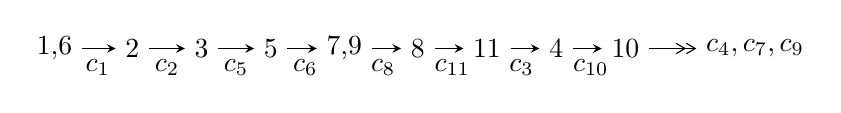
\begin{tikzpicture}[x=25pt, y=7pt]
	% node
	\node (A0) at (-1/8, 0) {1,6};
	\node (A1) at (1, 0) {2};
	\node (A2) at (2, 0) {3};
	\node (A3) at (3, 0) {5};
	\node (A4) at (65/16, 0) {7,9};
	\node (A5) at (41/8, 0) {8};
	\node (A6) at (49/8, 0) {11};
	\node (A7) at (57/8, 0) {4};
	\node (A8) at (65/8, 0) {10};
	\node (C1) at (1/2, -1) {$c_{1}$};
	\node (C2) at (3/2, -1) {$c_{2}$};
	\node (C3) at (5/2, -1) {$c_{5}$};
	\node (C4) at (7/2, -1) {$c_{6}$};
	\node (C5) at (37/8, -1) {$c_{8}$};
	\node (C6) at (45/8, -1) {$c_{11}$};
	\node (C7) at (53/8, -1) {$c_{3}$};
	\node (C8) at (61/8, -1) {$c_{10}$};
	\node (A9) at (10, 0) {$c_{4},c_{7},c_{9}$};

	% edge
	\draw[->,>=stealth]	
	(A0) edge (A1) (A1) edge (A2) (A2) edge (A3) (A3) edge (A4) (A4) edge (A5) (A5) edge (A6) (A6) edge (A7) (A7) edge (A8) ;
	\draw[->>,>={angle 60}]	
	(A8) edge (A9);
\end{tikzpicture} \\ 

\end{tabular} \\

\footnotetext{
The image of knot diagram is generated by the software ``\textbf{Draw programme}" developed by Andrew Bartholomew(\url{http://www.layer8.co.uk/maths/draw/index.htm\#Running-draw}), where we modified some parts for our purpose(\url{https://github.com/CATsTAILs/LinksPainter}).
}\phantom \\ \newline 
\centering \textbf{Ideals for irreducible components\footnotemark of $X_{\text{par}}$} 
 
\begin{align*}
I^u_{1}&=\langle 
-1271 u^{35}+7400 u^{34}+\cdots+559 b+6593,\;1511 u^{35}-17846 u^{34}+\cdots+2236 a-43197,\\
\phantom{I^u_{1}}&\phantom{= \langle  }u^{36}-6 u^{35}+\cdots+u+4\rangle \\
I^u_{2}&=\langle 
- u^{26} a+317 u^{26}+\cdots+a+1171,\;4 u^{26} a-3 u^{26}+\cdots-6 a+9,\;u^{27}+2 u^{26}+\cdots-4 u^2-1\rangle \\
I^u_{3}&=\langle 
-2 u^9+u^8-3 u^7+u^6-6 u^5+4 u^4-8 u^3+5 u^2+b-4 u+1,\;u^8+u^7+u^4+u^3- u^2+a-3,\\
\phantom{I^u_{3}}&\phantom{= \langle  }u^{10}- u^9+2 u^8- u^7+4 u^6-3 u^5+6 u^4-4 u^3+5 u^2- u+1\rangle \\
I^u_{4}&=\langle 
b+1,\;a^2-2 a u- a- u-2,\;u^2+u+1\rangle \\
\\
\end{align*}
\raggedright * 4 irreducible components of $\dim_{\mathbb{C}}=0$, with total 104 representations.\\
\footnotetext{All coefficients of polynomials are rational numbers. But the coefficients are sometimes approximated in decimal forms when there is not enough margin.}
\newpage
\renewcommand{\arraystretch}{1}
\centering \section*{I. $I^u_{1}= \langle -1271 u^{35}+7400 u^{34}+\cdots+559 b+6593,\;1511 u^{35}-17846 u^{34}+\cdots+2236 a-43197,\;u^{36}-6 u^{35}+\cdots+u+4 \rangle$}
\flushleft \textbf{(i) Arc colorings}\\
\begin{tabular}{m{7pt} m{180pt} m{7pt} m{180pt} }
\flushright $a_{1}=$&$\begin{pmatrix}1\\0\end{pmatrix}$ \\
\flushright $a_{6}=$&$\begin{pmatrix}0\\u\end{pmatrix}$ \\
\flushright $a_{2}=$&$\begin{pmatrix}1\\- u^2\end{pmatrix}$ \\
\flushright $a_{3}=$&$\begin{pmatrix}u^2+1\\- u^2\end{pmatrix}$ \\
\flushright $a_{5}=$&$\begin{pmatrix}- u\\u^3+u\end{pmatrix}$ \\
\flushright $a_{7}=$&$\begin{pmatrix}- u^3\\u^5+u^3+u\end{pmatrix}$ \\
\flushright $a_{9}=$&$\begin{pmatrix}-0.675760 u^{35}+7.98122 u^{34}+\cdots+27.4079 u+19.3189\\2.27370 u^{35}-13.2379 u^{34}+\cdots-13.8336 u-11.7943\end{pmatrix}$ \\
\flushright $a_{8}=$&$\begin{pmatrix}-5.13551 u^{35}+22.9168 u^{34}+\cdots-13.4794 u+0.555009\\11.4633 u^{35}-59.1413 u^{34}+\cdots+2.49732 u-22.1485\end{pmatrix}$ \\
\flushright $a_{11}=$&$\begin{pmatrix}2.05322 u^{35}-7.18515 u^{34}+\cdots+17.4490 u+7.42889\\-0.159213 u^{35}+0.654741 u^{34}+\cdots-7.64580 u-1.40072\end{pmatrix}$ \\
\flushright $a_{4}=$&$\begin{pmatrix}-4.34571 u^{35}+24.2531 u^{34}+\cdots+1.93202 u+12.1552\\1.29875 u^{35}-5.67800 u^{34}+\cdots+5.43649 u+1.81932\end{pmatrix}$ \\
\flushright $a_{10}=$&$\begin{pmatrix}5.53712 u^{35}-21.7594 u^{34}+\cdots+26.2039 u+8.03444\\-7.89624 u^{35}+42.0340 u^{34}+\cdots+5.69052 u+20.5420\end{pmatrix}$\\ \flushright $a_{10}=$&$\begin{pmatrix}5.53712 u^{35}-21.7594 u^{34}+\cdots+26.2039 u+8.03444\\-7.89624 u^{35}+42.0340 u^{34}+\cdots+5.69052 u+20.5420\end{pmatrix}$\\&\end{tabular}
\flushleft \textbf{(ii) Obstruction class $= -1$}\\~\\
\flushleft \textbf{(iii) Cusp Shapes $= \frac{4133}{559} u^{35}-\frac{18240}{559} u^{34}+\cdots+\frac{10119}{559} u-\frac{3554}{559}$}\\~\\
\newpage\renewcommand{\arraystretch}{1}
\flushleft \textbf{(iv) u-Polynomials at the component}\newline \\
\begin{tabular}{m{50pt}|m{274pt}}
Crossings & \hspace{64pt}u-Polynomials at each crossing \\
\hline $$\begin{aligned}c_{1},c_{5}\end{aligned}$$&$\begin{aligned}
&u^{36}-6 u^{35}+\cdots+u+4
\end{aligned}$\\
\hline $$\begin{aligned}c_{2},c_{6}\end{aligned}$$&$\begin{aligned}
&u^{36}+10 u^{35}+\cdots+31 u+16
\end{aligned}$\\
\hline $$\begin{aligned}c_{3},c_{7}\end{aligned}$$&$\begin{aligned}
&u^{36}+2 u^{35}+\cdots+2 u+1
\end{aligned}$\\
\hline $$\begin{aligned}c_{4},c_{8}\end{aligned}$$&$\begin{aligned}
&u^{36}+6 u^{34}+\cdots-5 u+2
\end{aligned}$\\
\hline $$\begin{aligned}c_{9},c_{11}\end{aligned}$$&$\begin{aligned}
&u^{36}+6 u^{35}+\cdots+4 u+1
\end{aligned}$\\
\hline $$\begin{aligned}c_{10}\end{aligned}$$&$\begin{aligned}
&u^{36}+19 u^{35}+\cdots+u+2
\end{aligned}$\\
\hline
\end{tabular}\\~\\
\newpage\renewcommand{\arraystretch}{1}
\flushleft \textbf{(v) Riley Polynomials at the component}\newline \\
\begin{tabular}{m{50pt}|m{274pt}}
Crossings & \hspace{64pt}Riley Polynomials at each crossing \\
\hline $$\begin{aligned}c_{1},c_{5}\end{aligned}$$&$\begin{aligned}
&y^{36}+10 y^{35}+\cdots+31 y+16
\end{aligned}$\\
\hline $$\begin{aligned}c_{2},c_{6}\end{aligned}$$&$\begin{aligned}
&y^{36}+34 y^{35}+\cdots-6849 y+256
\end{aligned}$\\
\hline $$\begin{aligned}c_{3},c_{7}\end{aligned}$$&$\begin{aligned}
&y^{36}+24 y^{35}+\cdots+44 y+1
\end{aligned}$\\
\hline $$\begin{aligned}c_{4},c_{8}\end{aligned}$$&$\begin{aligned}
&y^{36}+12 y^{35}+\cdots+27 y+4
\end{aligned}$\\
\hline $$\begin{aligned}c_{9},c_{11}\end{aligned}$$&$\begin{aligned}
&y^{36}-8 y^{35}+\cdots+28 y+1
\end{aligned}$\\
\hline $$\begin{aligned}c_{10}\end{aligned}$$&$\begin{aligned}
&y^{36}- y^{35}+\cdots+67 y+4
\end{aligned}$\\
\hline
\end{tabular}\\~\\
\newpage\flushleft \textbf{(vi) Complex Volumes and Cusp Shapes}
$$\begin{array}{c|c|c}  
\text{Solutions to }I^u_{1}& \I (\text{vol} + \sqrt{-1}CS) & \text{Cusp shape}\\
 \hline 
\begin{aligned}
u &= -0.276741 + 0.944175 I \\
a &= -1.25934 + 0.87235 I \\
b &= -1.18704 - 0.84945 I\end{aligned}
 & -3.77194 - 4.33449 I & -10.34773 + 8.70742 I \\ \hline\begin{aligned}
u &= -0.276741 - 0.944175 I \\
a &= -1.25934 - 0.87235 I \\
b &= -1.18704 + 0.84945 I\end{aligned}
 & -3.77194 + 4.33449 I & -10.34773 - 8.70742 I \\ \hline\begin{aligned}
u &= -0.304491 + 0.889790 I \\
a &= -0.062800 + 1.255710 I \\
b &= -1.142480 + 0.222558 I\end{aligned}
 & -3.69796 - 0.78585 I & -10.32257 + 1.08257 I \\ \hline\begin{aligned}
u &= -0.304491 - 0.889790 I \\
a &= -0.062800 - 1.255710 I \\
b &= -1.142480 - 0.222558 I\end{aligned}
 & -3.69796 + 0.78585 I & -10.32257 - 1.08257 I \\ \hline\begin{aligned}
u &= \phantom{-}0.700901 + 0.854931 I \\
a &= \phantom{-}0.21075 - 1.52850 I \\
b &= -0.322329 + 0.571982 I\end{aligned}
 & \phantom{-}0.84484 + 3.07899 I & -2.36753 - 4.61435 I \\ \hline\begin{aligned}
u &= \phantom{-}0.700901 - 0.854931 I \\
a &= \phantom{-}0.21075 + 1.52850 I \\
b &= -0.322329 - 0.571982 I\end{aligned}
 & \phantom{-}0.84484 - 3.07899 I & -2.36753 + 4.61435 I \\ \hline\begin{aligned}
u &= \phantom{-}0.670636 + 0.904481 I \\
a &= \phantom{-}0.853772 + 0.895928 I \\
b &= -0.023486 - 0.449791 I\end{aligned}
 & \phantom{-}0.69868 + 2.21160 I & -2.61972 - 2.06632 I \\ \hline\begin{aligned}
u &= \phantom{-}0.670636 - 0.904481 I \\
a &= \phantom{-}0.853772 - 0.895928 I \\
b &= -0.023486 + 0.449791 I\end{aligned}
 & \phantom{-}0.69868 - 2.21160 I & -2.61972 + 2.06632 I \\ \hline\begin{aligned}
u &= -0.848515 + 0.073137 I \\
a &= -0.708084 + 0.620130 I \\
b &= \phantom{-}0.741423 - 0.831359 I\end{aligned}
 & \phantom{-}1.04891 + 7.93873 I & \phantom{-}2.26099 - 7.53856 I \\ \hline\begin{aligned}
u &= -0.848515 - 0.073137 I \\
a &= -0.708084 - 0.620130 I \\
b &= \phantom{-}0.741423 + 0.831359 I\end{aligned}
 & \phantom{-}1.04891 - 7.93873 I & \phantom{-}2.26099 + 7.53856 I\\
 \hline 
 \end{array}$$\newpage$$\begin{array}{c|c|c}  
\text{Solutions to }I^u_{1}& \I (\text{vol} + \sqrt{-1}CS) & \text{Cusp shape}\\
 \hline 
\begin{aligned}
u &= -0.335316 + 1.103160 I \\
a &= \phantom{-}0.986796 - 0.482008 I \\
b &= \phantom{-}1.076210 + 0.827984 I\end{aligned}
 & -2.43737 - 11.97940 I & -3.58846 + 9.69532 I \\ \hline\begin{aligned}
u &= -0.335316 - 1.103160 I \\
a &= \phantom{-}0.986796 + 0.482008 I \\
b &= \phantom{-}1.076210 - 0.827984 I\end{aligned}
 & -2.43737 + 11.97940 I & -3.58846 - 9.69532 I \\ \hline\begin{aligned}
u &= -0.754047 + 0.880053 I \\
a &= \phantom{-}0.256067 + 0.953865 I \\
b &= -1.57066 + 0.07535 I\end{aligned}
 & \phantom{-}1.51994 - 2.85709 I & -2.33106 + 2.86602 I \\ \hline\begin{aligned}
u &= -0.754047 - 0.880053 I \\
a &= \phantom{-}0.256067 - 0.953865 I \\
b &= -1.57066 - 0.07535 I\end{aligned}
 & \phantom{-}1.51994 + 2.85709 I & -2.33106 - 2.86602 I \\ \hline\begin{aligned}
u &= \phantom{-}0.836947 + 0.813811 I \\
a &= \phantom{-}1.45743 + 1.45510 I \\
b &= -0.90494 - 1.42986 I\end{aligned}
 & \phantom{-}3.28088 - 2.39771 I & -4.49853 + 2.73594 I \\ \hline\begin{aligned}
u &= \phantom{-}0.836947 - 0.813811 I \\
a &= \phantom{-}1.45743 - 1.45510 I \\
b &= -0.90494 + 1.42986 I\end{aligned}
 & \phantom{-}3.28088 + 2.39771 I & -4.49853 - 2.73594 I \\ \hline\begin{aligned}
u &= -0.185132 + 1.158740 I \\
a &= \phantom{-}0.116551 - 0.668626 I \\
b &= \phantom{-}0.655109 - 0.395481 I\end{aligned}
 & -3.33480 + 4.43993 I & -6.66340 - 7.47745 I \\ \hline\begin{aligned}
u &= -0.185132 - 1.158740 I \\
a &= \phantom{-}0.116551 + 0.668626 I \\
b &= \phantom{-}0.655109 + 0.395481 I\end{aligned}
 & -3.33480 - 4.43993 I & -6.66340 + 7.47745 I \\ \hline\begin{aligned}
u &= \phantom{-}0.911501 + 0.758905 I \\
a &= -1.10120 - 1.05489 I \\
b &= \phantom{-}1.12689 + 1.25578 I\end{aligned}
 & \phantom{-}5.92417 - 11.34300 I & \phantom{-}2.20430 + 5.55458 I \\ \hline\begin{aligned}
u &= \phantom{-}0.911501 - 0.758905 I \\
a &= -1.10120 + 1.05489 I \\
b &= \phantom{-}1.12689 - 1.25578 I\end{aligned}
 & \phantom{-}5.92417 + 11.34300 I & \phantom{-}2.20430 - 5.55458 I\\
 \hline 
 \end{array}$$\newpage$$\begin{array}{c|c|c}  
\text{Solutions to }I^u_{1}& \I (\text{vol} + \sqrt{-1}CS) & \text{Cusp shape}\\
 \hline 
\begin{aligned}
u &= -0.824017 + 0.898169 I \\
a &= -0.177149 - 0.497820 I \\
b &= \phantom{-}0.921405 - 0.086126 I\end{aligned}
 & \phantom{-}6.48061 - 3.07379 I & \phantom{-}6.45709 + 2.41299 I \\ \hline\begin{aligned}
u &= -0.824017 - 0.898169 I \\
a &= -0.177149 + 0.497820 I \\
b &= \phantom{-}0.921405 + 0.086126 I\end{aligned}
 & \phantom{-}6.48061 + 3.07379 I & \phantom{-}6.45709 - 2.41299 I \\ \hline\begin{aligned}
u &= \phantom{-}0.021281 + 0.766965 I \\
a &= -1.40357 + 1.58774 I \\
b &= -1.045680 - 0.299865 I\end{aligned}
 & -2.80406 + 0.04358 I & -9.18489 + 0.34635 I \\ \hline\begin{aligned}
u &= \phantom{-}0.021281 - 0.766965 I \\
a &= -1.40357 - 1.58774 I \\
b &= -1.045680 + 0.299865 I\end{aligned}
 & -2.80406 - 0.04358 I & -9.18489 - 0.34635 I \\ \hline\begin{aligned}
u &= \phantom{-}0.789000 + 0.963507 I \\
a &= -0.51131 - 2.47418 I \\
b &= -1.06736 + 1.45192 I\end{aligned}
 & \phantom{-}2.81727 + 8.47181 I & -5.83967 - 8.29612 I \\ \hline\begin{aligned}
u &= \phantom{-}0.789000 - 0.963507 I \\
a &= -0.51131 + 2.47418 I \\
b &= -1.06736 - 1.45192 I\end{aligned}
 & \phantom{-}2.81727 - 8.47181 I & -5.83967 + 8.29612 I \\ \hline\begin{aligned}
u &= \phantom{-}0.374008 + 0.626804 I \\
a &= \phantom{-}0.891587 - 0.075576 I \\
b &= \phantom{-}0.070132 + 0.290278 I\end{aligned}
 & \phantom{-}0.10177 + 1.47413 I & \phantom{-}1.25501 - 4.83821 I \\ \hline\begin{aligned}
u &= \phantom{-}0.374008 - 0.626804 I \\
a &= \phantom{-}0.891587 + 0.075576 I \\
b &= \phantom{-}0.070132 - 0.290278 I\end{aligned}
 & \phantom{-}0.10177 - 1.47413 I & \phantom{-}1.25501 + 4.83821 I \\ \hline\begin{aligned}
u &= \phantom{-}1.028740 + 0.773325 I \\
a &= \phantom{-}0.187909 + 0.308356 I \\
b &= -0.190982 - 0.521409 I\end{aligned}
 & \phantom{-}4.99883 + 3.21347 I & \phantom{-}19.6525 + 3.8446 I \\ \hline\begin{aligned}
u &= \phantom{-}1.028740 - 0.773325 I \\
a &= \phantom{-}0.187909 - 0.308356 I \\
b &= -0.190982 + 0.521409 I\end{aligned}
 & \phantom{-}4.99883 - 3.21347 I & \phantom{-}19.6525 - 3.8446 I\\
 \hline 
 \end{array}$$\newpage$$\begin{array}{c|c|c}  
\text{Solutions to }I^u_{1}& \I (\text{vol} + \sqrt{-1}CS) & \text{Cusp shape}\\
 \hline 
\begin{aligned}
u &= \phantom{-}0.798120 + 1.025270 I \\
a &= \phantom{-}0.57651 + 2.10645 I \\
b &= \phantom{-}1.23838 - 1.24673 I\end{aligned}
 & \phantom{-}5.0855 + 17.6564 I & \phantom{-}0.86604 - 10.01914 I \\ \hline\begin{aligned}
u &= \phantom{-}0.798120 - 1.025270 I \\
a &= \phantom{-}0.57651 - 2.10645 I \\
b &= \phantom{-}1.23838 + 1.24673 I\end{aligned}
 & \phantom{-}5.0855 - 17.6564 I & \phantom{-}0.86604 + 10.01914 I \\ \hline\begin{aligned}
u &= \phantom{-}0.880565 + 1.020470 I \\
a &= \phantom{-}0.032721 - 0.717303 I \\
b &= -0.616024 + 0.418194 I\end{aligned}
 & \phantom{-}4.23977 + 3.68667 I & \phantom{-0.000000 } 0. - 11.71183 I \\ \hline\begin{aligned}
u &= \phantom{-}0.880565 - 1.020470 I \\
a &= \phantom{-}0.032721 + 0.717303 I \\
b &= -0.616024 - 0.418194 I\end{aligned}
 & \phantom{-}4.23977 - 3.68667 I & \phantom{-0.000000 -}0. + 11.71183 I \\ \hline\begin{aligned}
u &= -0.483436 + 0.080826 I \\
a &= \phantom{-}1.52835 - 0.78222 I \\
b &= -0.758556 + 0.609588 I\end{aligned}
 & -1.25585 + 1.57291 I & -2.37601 - 4.05394 I \\ \hline\begin{aligned}
u &= -0.483436 - 0.080826 I \\
a &= \phantom{-}1.52835 + 0.78222 I \\
b &= -0.758556 - 0.609588 I\end{aligned}
 & -1.25585 - 1.57291 I & -2.37601 + 4.05394 I\\
 \hline 
 \end{array}$$\newpage\newpage\renewcommand{\arraystretch}{1}
\centering \section*{II. $I^u_{2}= \langle - u^{26} a+317 u^{26}+\cdots+a+1171,\;4 u^{26} a-3 u^{26}+\cdots-6 a+9,\;u^{27}+2 u^{26}+\cdots-4 u^2-1 \rangle$}
\flushleft \textbf{(i) Arc colorings}\\
\begin{tabular}{m{7pt} m{180pt} m{7pt} m{180pt} }
\flushright $a_{1}=$&$\begin{pmatrix}1\\0\end{pmatrix}$ \\
\flushright $a_{6}=$&$\begin{pmatrix}0\\u\end{pmatrix}$ \\
\flushright $a_{2}=$&$\begin{pmatrix}1\\- u^2\end{pmatrix}$ \\
\flushright $a_{3}=$&$\begin{pmatrix}u^2+1\\- u^2\end{pmatrix}$ \\
\flushright $a_{5}=$&$\begin{pmatrix}- u\\u^3+u\end{pmatrix}$ \\
\flushright $a_{7}=$&$\begin{pmatrix}- u^3\\u^5+u^3+u\end{pmatrix}$ \\
\flushright $a_{9}=$&$\begin{pmatrix}a\\0.00201613 a u^{26}-0.639113 u^{26}+\cdots-0.00201613 a-2.36089\end{pmatrix}$ \\
\flushright $a_{8}=$&$\begin{pmatrix}0.00806452 a u^{26}-1.55645 u^{26}+\cdots+0.991935 a+0.556452\\-0.00201613 a u^{26}-0.360887 u^{26}+\cdots+0.00201613 a-3.63911\end{pmatrix}$ \\
\flushright $a_{11}=$&$\begin{pmatrix}0.360887 a u^{26}+2.59879 u^{26}+\cdots+0.639113 a+0.401210\\0.917339 a u^{26}-0.796371 u^{26}+\cdots-0.917339 a+3.79637\end{pmatrix}$ \\
\flushright $a_{4}=$&$\begin{pmatrix}1.08266 a u^{26}-3.20363 u^{26}+\cdots-0.0826613 a+2.20363\\-0.0524194 a u^{26}-0.383065 u^{26}+\cdots+1.05242 a+1.38306\end{pmatrix}$ \\
\flushright $a_{10}=$&$\begin{pmatrix}-0.00201613 a u^{26}-0.360887 u^{26}+\cdots+1.00202 a+0.360887\\0.00806452 a u^{26}+0.443548 u^{26}+\cdots-0.00806452 a-3.44355\end{pmatrix}$\\ \flushright $a_{10}=$&$\begin{pmatrix}-0.00201613 a u^{26}-0.360887 u^{26}+\cdots+1.00202 a+0.360887\\0.00806452 a u^{26}+0.443548 u^{26}+\cdots-0.00806452 a-3.44355\end{pmatrix}$\\&\end{tabular}
\flushleft \textbf{(ii) Obstruction class $= -1$}\\~\\
\flushleft \textbf{(iii) Cusp Shapes $= 3 u^{26}+5 u^{24}- u^{23}+18 u^{22}-8 u^{21}+17 u^{20}-8 u^{19}+27 u^{18}-30 u^{17}+9 u^{16}+2 u^{15}-8 u^{14}-4 u^{13}-14 u^{12}+64 u^{11}-52 u^{10}+70 u^9-24 u^8+71 u^7-52 u^6+46 u^5-25 u^4+2 u^3-11 u^2+2 u+3$}\\~\\
\newpage\renewcommand{\arraystretch}{1}
\flushleft \textbf{(iv) u-Polynomials at the component}\newline \\
\begin{tabular}{m{50pt}|m{274pt}}
Crossings & \hspace{64pt}u-Polynomials at each crossing \\
\hline $$\begin{aligned}c_{1},c_{5}\end{aligned}$$&$\begin{aligned}
&(u^{27}+2 u^{26}+\cdots-4 u^2-1)^{2}
\end{aligned}$\\
\hline $$\begin{aligned}c_{2},c_{6}\end{aligned}$$&$\begin{aligned}
&(u^{27}+8 u^{26}+\cdots-8 u-1)^{2}
\end{aligned}$\\
\hline $$\begin{aligned}c_{3},c_{7}\end{aligned}$$&$\begin{aligned}
&u^{54}+4 u^{53}+\cdots+9 u+2
\end{aligned}$\\
\hline $$\begin{aligned}c_{4},c_{8}\end{aligned}$$&$\begin{aligned}
&u^{54}+2 u^{53}+\cdots-1697 u+407
\end{aligned}$\\
\hline $$\begin{aligned}c_{9},c_{11}\end{aligned}$$&$\begin{aligned}
&u^{54}-5 u^{53}+\cdots-529 u+44
\end{aligned}$\\
\hline $$\begin{aligned}c_{10}\end{aligned}$$&$\begin{aligned}
&(u^{27}-13 u^{26}+\cdots-10 u+4)^{2}
\end{aligned}$\\
\hline
\end{tabular}\\~\\
\newpage\renewcommand{\arraystretch}{1}
\flushleft \textbf{(v) Riley Polynomials at the component}\newline \\
\begin{tabular}{m{50pt}|m{274pt}}
Crossings & \hspace{64pt}Riley Polynomials at each crossing \\
\hline $$\begin{aligned}c_{1},c_{5}\end{aligned}$$&$\begin{aligned}
&(y^{27}+8 y^{26}+\cdots-8 y-1)^{2}
\end{aligned}$\\
\hline $$\begin{aligned}c_{2},c_{6}\end{aligned}$$&$\begin{aligned}
&(y^{27}+24 y^{26}+\cdots-12 y-1)^{2}
\end{aligned}$\\
\hline $$\begin{aligned}c_{3},c_{7}\end{aligned}$$&$\begin{aligned}
&y^{54}-8 y^{53}+\cdots+87 y+4
\end{aligned}$\\
\hline $$\begin{aligned}c_{4},c_{8}\end{aligned}$$&$\begin{aligned}
&y^{54}+12 y^{53}+\cdots+4226411 y+165649
\end{aligned}$\\
\hline $$\begin{aligned}c_{9},c_{11}\end{aligned}$$&$\begin{aligned}
&y^{54}+23 y^{53}+\cdots+25783 y+1936
\end{aligned}$\\
\hline $$\begin{aligned}c_{10}\end{aligned}$$&$\begin{aligned}
&(y^{27}-5 y^{26}+\cdots+236 y-16)^{2}
\end{aligned}$\\
\hline
\end{tabular}\\~\\
\newpage\flushleft \textbf{(vi) Complex Volumes and Cusp Shapes}
$$\begin{array}{c|c|c}  
\text{Solutions to }I^u_{2}& \I (\text{vol} + \sqrt{-1}CS) & \text{Cusp shape}\\
 \hline 
\begin{aligned}
u &= \phantom{-}0.144711 + 0.987236 I \\
a &= -1.044320 + 0.252570 I \\
b &= -1.10548 + 0.93118 I\end{aligned}
 & -3.43692 + 4.10370 I & -10.33067 - 7.76154 I \\ \hline\begin{aligned}
u &= \phantom{-}0.144711 + 0.987236 I \\
a &= \phantom{-}1.17591 + 1.35422 I \\
b &= \phantom{-}0.694713 - 0.161571 I\end{aligned}
 & -3.43692 + 4.10370 I & -10.33067 - 7.76154 I \\ \hline\begin{aligned}
u &= \phantom{-}0.144711 - 0.987236 I \\
a &= -1.044320 - 0.252570 I \\
b &= -1.10548 - 0.93118 I\end{aligned}
 & -3.43692 - 4.10370 I & -10.33067 + 7.76154 I \\ \hline\begin{aligned}
u &= \phantom{-}0.144711 - 0.987236 I \\
a &= \phantom{-}1.17591 - 1.35422 I \\
b &= \phantom{-}0.694713 + 0.161571 I\end{aligned}
 & -3.43692 - 4.10370 I & -10.33067 + 7.76154 I \\ \hline\begin{aligned}
u &= \phantom{-}0.504183 + 0.966350 I \\
a &= \phantom{-}0.867903 + 0.476539 I \\
b &= \phantom{-}0.929423 + 0.017439 I\end{aligned}
 & -1.43447 + 1.57559 I & -0.45968 + 6.99556 I \\ \hline\begin{aligned}
u &= \phantom{-}0.504183 + 0.966350 I \\
a &= \phantom{-}0.992670 - 0.899903 I \\
b &= -0.809221 - 0.348625 I\end{aligned}
 & -1.43447 + 1.57559 I & -0.45968 + 6.99556 I \\ \hline\begin{aligned}
u &= \phantom{-}0.504183 - 0.966350 I \\
a &= \phantom{-}0.867903 - 0.476539 I \\
b &= \phantom{-}0.929423 - 0.017439 I\end{aligned}
 & -1.43447 - 1.57559 I & -0.45968 - 6.99556 I \\ \hline\begin{aligned}
u &= \phantom{-}0.504183 - 0.966350 I \\
a &= \phantom{-}0.992670 + 0.899903 I \\
b &= -0.809221 + 0.348625 I\end{aligned}
 & -1.43447 - 1.57559 I & -0.45968 - 6.99556 I \\ \hline\begin{aligned}
u &= -0.770533 + 0.784290 I \\
a &= -0.44956 + 1.58387 I \\
b &= \phantom{-}0.151642 - 0.255883 I\end{aligned}
 & \phantom{-}2.45928 + 3.09185 I & -2.04409 - 4.31047 I \\ \hline\begin{aligned}
u &= -0.770533 + 0.784290 I \\
a &= \phantom{-}1.53553 - 1.36774 I \\
b &= -1.00807 + 1.68610 I\end{aligned}
 & \phantom{-}2.45928 + 3.09185 I & -2.04409 - 4.31047 I\\
 \hline 
 \end{array}$$\newpage$$\begin{array}{c|c|c}  
\text{Solutions to }I^u_{2}& \I (\text{vol} + \sqrt{-1}CS) & \text{Cusp shape}\\
 \hline 
\begin{aligned}
u &= -0.770533 - 0.784290 I \\
a &= -0.44956 - 1.58387 I \\
b &= \phantom{-}0.151642 + 0.255883 I\end{aligned}
 & \phantom{-}2.45928 - 3.09185 I & -2.04409 + 4.31047 I \\ \hline\begin{aligned}
u &= -0.770533 - 0.784290 I \\
a &= \phantom{-}1.53553 + 1.36774 I \\
b &= -1.00807 - 1.68610 I\end{aligned}
 & \phantom{-}2.45928 - 3.09185 I & -2.04409 + 4.31047 I \\ \hline\begin{aligned}
u &= \phantom{-}0.291946 + 1.107070 I \\
a &= \phantom{-}0.931124 + 0.230119 I \\
b &= \phantom{-}0.646966 - 0.516614 I\end{aligned}
 & -0.60671 + 3.68820 I & \phantom{-}4.86231 - 6.92207 I \\ \hline\begin{aligned}
u &= \phantom{-}0.291946 + 1.107070 I \\
a &= -0.323787 + 0.014224 I \\
b &= -0.311394 + 0.647844 I\end{aligned}
 & -0.60671 + 3.68820 I & \phantom{-}4.86231 - 6.92207 I \\ \hline\begin{aligned}
u &= \phantom{-}0.291946 - 1.107070 I \\
a &= \phantom{-}0.931124 - 0.230119 I \\
b &= \phantom{-}0.646966 + 0.516614 I\end{aligned}
 & -0.60671 - 3.68820 I & \phantom{-}4.86231 + 6.92207 I \\ \hline\begin{aligned}
u &= \phantom{-}0.291946 - 1.107070 I \\
a &= -0.323787 - 0.014224 I \\
b &= -0.311394 - 0.647844 I\end{aligned}
 & -0.60671 - 3.68820 I & \phantom{-}4.86231 + 6.92207 I \\ \hline\begin{aligned}
u &= -0.898179 + 0.746104 I \\
a &= -0.594838 + 0.861512 I \\
b &= \phantom{-}0.874324 - 0.984284 I\end{aligned}
 & \phantom{-}7.41344 + 3.23384 I & \phantom{-}5.98510 - 2.95350 I \\ \hline\begin{aligned}
u &= -0.898179 + 0.746104 I \\
a &= \phantom{-}0.595344 - 1.207400 I \\
b &= -0.349108 + 1.259600 I\end{aligned}
 & \phantom{-}7.41344 + 3.23384 I & \phantom{-}5.98510 - 2.95350 I \\ \hline\begin{aligned}
u &= -0.898179 - 0.746104 I \\
a &= -0.594838 - 0.861512 I \\
b &= \phantom{-}0.874324 + 0.984284 I\end{aligned}
 & \phantom{-}7.41344 - 3.23384 I & \phantom{-}5.98510 + 2.95350 I \\ \hline\begin{aligned}
u &= -0.898179 - 0.746104 I \\
a &= \phantom{-}0.595344 + 1.207400 I \\
b &= -0.349108 - 1.259600 I\end{aligned}
 & \phantom{-}7.41344 - 3.23384 I & \phantom{-}5.98510 + 2.95350 I\\
 \hline 
 \end{array}$$\newpage$$\begin{array}{c|c|c}  
\text{Solutions to }I^u_{2}& \I (\text{vol} + \sqrt{-1}CS) & \text{Cusp shape}\\
 \hline 
\begin{aligned}
u &= \phantom{-}0.799598 + 0.863452 I \\
a &= \phantom{-}0.472052 + 1.331300 I \\
b &= -0.753138 - 1.063980 I\end{aligned}
 & \phantom{-}5.90777 - 1.53174 I & \phantom{-}5.51904 + 2.02847 I \\ \hline\begin{aligned}
u &= \phantom{-}0.799598 + 0.863452 I \\
a &= \phantom{-}0.53604 + 2.57871 I \\
b &= \phantom{-}1.21139 - 1.71770 I\end{aligned}
 & \phantom{-}5.90777 - 1.53174 I & \phantom{-}5.51904 + 2.02847 I \\ \hline\begin{aligned}
u &= \phantom{-}0.799598 - 0.863452 I \\
a &= \phantom{-}0.472052 - 1.331300 I \\
b &= -0.753138 + 1.063980 I\end{aligned}
 & \phantom{-}5.90777 + 1.53174 I & \phantom{-}5.51904 - 2.02847 I \\ \hline\begin{aligned}
u &= \phantom{-}0.799598 - 0.863452 I \\
a &= \phantom{-}0.53604 - 2.57871 I \\
b &= \phantom{-}1.21139 + 1.71770 I\end{aligned}
 & \phantom{-}5.90777 + 1.53174 I & \phantom{-}5.51904 - 2.02847 I \\ \hline\begin{aligned}
u &= \phantom{-}0.802525\phantom{ +0.000000I} \\
a &= \phantom{-}0.064178 + 0.713542 I \\
b &= \phantom{-}0.219481 - 0.777240 I\end{aligned}
 & \phantom{-}3.09479\phantom{ +0.000000I} & \phantom{-}9.01780\phantom{ +0.000000I} \\ \hline\begin{aligned}
u &= \phantom{-}0.802525\phantom{ +0.000000I} \\
a &= \phantom{-}0.064178 - 0.713542 I \\
b &= \phantom{-}0.219481 + 0.777240 I\end{aligned}
 & \phantom{-}3.09479\phantom{ +0.000000I} & \phantom{-}9.01780\phantom{ +0.000000I} \\ \hline\begin{aligned}
u &= \phantom{-}0.785462 + 0.911233 I \\
a &= -1.79873 - 1.10105 I \\
b &= \phantom{-}1.09759 + 1.87961 I\end{aligned}
 & \phantom{-}5.75923 + 7.48234 I & \phantom{-}4.88411 - 7.87589 I \\ \hline\begin{aligned}
u &= \phantom{-}0.785462 + 0.911233 I \\
a &= -1.04193 - 2.09558 I \\
b &= -0.810627 + 0.965025 I\end{aligned}
 & \phantom{-}5.75923 + 7.48234 I & \phantom{-}4.88411 - 7.87589 I \\ \hline\begin{aligned}
u &= \phantom{-}0.785462 - 0.911233 I \\
a &= -1.79873 + 1.10105 I \\
b &= \phantom{-}1.09759 - 1.87961 I\end{aligned}
 & \phantom{-}5.75923 - 7.48234 I & \phantom{-}4.88411 + 7.87589 I \\ \hline\begin{aligned}
u &= \phantom{-}0.785462 - 0.911233 I \\
a &= -1.04193 + 2.09558 I \\
b &= -0.810627 - 0.965025 I\end{aligned}
 & \phantom{-}5.75923 - 7.48234 I & \phantom{-}4.88411 + 7.87589 I\\
 \hline 
 \end{array}$$\newpage$$\begin{array}{c|c|c}  
\text{Solutions to }I^u_{2}& \I (\text{vol} + \sqrt{-1}CS) & \text{Cusp shape}\\
 \hline 
\begin{aligned}
u &= -0.740227 + 0.958313 I \\
a &= \phantom{-}0.17325 - 1.77767 I \\
b &= \phantom{-}0.279114 + 0.386141 I\end{aligned}
 & \phantom{-}1.92805 - 8.81809 I & -3.51760 + 9.35403 I \\ \hline\begin{aligned}
u &= -0.740227 + 0.958313 I \\
a &= -0.83078 + 2.42491 I \\
b &= -1.23050 - 1.60076 I\end{aligned}
 & \phantom{-}1.92805 - 8.81809 I & -3.51760 + 9.35403 I \\ \hline\begin{aligned}
u &= -0.740227 - 0.958313 I \\
a &= \phantom{-}0.17325 + 1.77767 I \\
b &= \phantom{-}0.279114 - 0.386141 I\end{aligned}
 & \phantom{-}1.92805 + 8.81809 I & -3.51760 - 9.35403 I \\ \hline\begin{aligned}
u &= -0.740227 - 0.958313 I \\
a &= -0.83078 - 2.42491 I \\
b &= -1.23050 + 1.60076 I\end{aligned}
 & \phantom{-}1.92805 + 8.81809 I & -3.51760 - 9.35403 I \\ \hline\begin{aligned}
u &= -0.818350 + 0.893459 I \\
a &= \phantom{-}0.013291 - 1.076530 I \\
b &= \phantom{-}1.005790 + 0.379819 I\end{aligned}
 & \phantom{-}6.46144 - 3.05379 I & \phantom{-}5.97423 + 2.71426 I \\ \hline\begin{aligned}
u &= -0.818350 + 0.893459 I \\
a &= -0.350459 + 0.093702 I \\
b &= \phantom{-}0.789809 - 0.525186 I\end{aligned}
 & \phantom{-}6.46144 - 3.05379 I & \phantom{-}5.97423 + 2.71426 I \\ \hline\begin{aligned}
u &= -0.818350 - 0.893459 I \\
a &= \phantom{-}0.013291 + 1.076530 I \\
b &= \phantom{-}1.005790 - 0.379819 I\end{aligned}
 & \phantom{-}6.46144 + 3.05379 I & \phantom{-}5.97423 - 2.71426 I \\ \hline\begin{aligned}
u &= -0.818350 - 0.893459 I \\
a &= -0.350459 - 0.093702 I \\
b &= \phantom{-}0.789809 + 0.525186 I\end{aligned}
 & \phantom{-}6.46144 + 3.05379 I & \phantom{-}5.97423 - 2.71426 I \\ \hline\begin{aligned}
u &= -0.194164 + 0.737666 I \\
a &= -0.1051250 - 0.0794208 I \\
b &= \phantom{-}0.24714 - 1.64517 I\end{aligned}
 & \phantom{-}0.15408 - 4.76928 I & -1.41513 + 11.31767 I \\ \hline\begin{aligned}
u &= -0.194164 + 0.737666 I \\
a &= -3.27600 - 0.27489 I \\
b &= -0.393595 - 0.629207 I\end{aligned}
 & \phantom{-}0.15408 - 4.76928 I & -1.41513 + 11.31767 I\\
 \hline 
 \end{array}$$\newpage$$\begin{array}{c|c|c}  
\text{Solutions to }I^u_{2}& \I (\text{vol} + \sqrt{-1}CS) & \text{Cusp shape}\\
 \hline 
\begin{aligned}
u &= -0.194164 - 0.737666 I \\
a &= -0.1051250 + 0.0794208 I \\
b &= \phantom{-}0.24714 + 1.64517 I\end{aligned}
 & \phantom{-}0.15408 + 4.76928 I & -1.41513 - 11.31767 I \\ \hline\begin{aligned}
u &= -0.194164 - 0.737666 I \\
a &= -3.27600 + 0.27489 I \\
b &= -0.393595 + 0.629207 I\end{aligned}
 & \phantom{-}0.15408 + 4.76928 I & -1.41513 - 11.31767 I \\ \hline\begin{aligned}
u &= -0.786810 + 1.024740 I \\
a &= -0.87495 + 1.40397 I \\
b &= -0.499560 - 1.264320 I\end{aligned}
 & \phantom{-}6.54280 - 9.46925 I & \phantom{-}4.33045 + 8.20563 I \\ \hline\begin{aligned}
u &= -0.786810 + 1.024740 I \\
a &= \phantom{-}0.67436 - 1.65262 I \\
b &= \phantom{-}0.990241 + 0.929170 I\end{aligned}
 & \phantom{-}6.54280 - 9.46925 I & \phantom{-}4.33045 + 8.20563 I \\ \hline\begin{aligned}
u &= -0.786810 - 1.024740 I \\
a &= -0.87495 - 1.40397 I \\
b &= -0.499560 + 1.264320 I\end{aligned}
 & \phantom{-}6.54280 + 9.46925 I & \phantom{-}4.33045 - 8.20563 I \\ \hline\begin{aligned}
u &= -0.786810 - 1.024740 I \\
a &= \phantom{-}0.67436 + 1.65262 I \\
b &= \phantom{-}0.990241 - 0.929170 I\end{aligned}
 & \phantom{-}6.54280 + 9.46925 I & \phantom{-}4.33045 - 8.20563 I \\ \hline\begin{aligned}
u &= \phantom{-}0.522984 + 0.315101 I \\
a &= \phantom{-}0.220722 + 1.030080 I \\
b &= \phantom{-}0.852048 + 0.137605 I\end{aligned}
 & \phantom{-}0.23096 + 2.37565 I & \phantom{-}1.69627 - 5.05605 I \\ \hline\begin{aligned}
u &= \phantom{-}0.522984 + 0.315101 I \\
a &= \phantom{-}1.14627 - 0.90462 I \\
b &= -0.541670 + 0.765569 I\end{aligned}
 & \phantom{-}0.23096 + 2.37565 I & \phantom{-}1.69627 - 5.05605 I \\ \hline\begin{aligned}
u &= \phantom{-}0.522984 - 0.315101 I \\
a &= \phantom{-}0.220722 - 1.030080 I \\
b &= \phantom{-}0.852048 - 0.137605 I\end{aligned}
 & \phantom{-}0.23096 - 2.37565 I & \phantom{-}1.69627 + 5.05605 I \\ \hline\begin{aligned}
u &= \phantom{-}0.522984 - 0.315101 I \\
a &= \phantom{-}1.14627 + 0.90462 I \\
b &= -0.541670 - 0.765569 I\end{aligned}
 & \phantom{-}0.23096 - 2.37565 I & \phantom{-}1.69627 + 5.05605 I\\
 \hline 
 \end{array}$$\newpage$$\begin{array}{c|c|c}  
\text{Solutions to }I^u_{2}& \I (\text{vol} + \sqrt{-1}CS) & \text{Cusp shape}\\
 \hline 
\begin{aligned}
u &= -0.241884 + 0.503654 I \\
a &= \phantom{-}0.93986 - 1.89203 I \\
b &= -0.363999 + 1.059620 I\end{aligned}
 & \phantom{-}0.79481 + 2.83207 I & \phantom{-}2.50674 + 1.28047 I \\ \hline\begin{aligned}
u &= -0.241884 + 0.503654 I \\
a &= \phantom{-}2.35199 + 0.56436 I \\
b &= \phantom{-}0.686698 + 0.816102 I\end{aligned}
 & \phantom{-}0.79481 + 2.83207 I & \phantom{-}2.50674 + 1.28047 I \\ \hline\begin{aligned}
u &= -0.241884 - 0.503654 I \\
a &= \phantom{-}0.93986 + 1.89203 I \\
b &= -0.363999 - 1.059620 I\end{aligned}
 & \phantom{-}0.79481 - 2.83207 I & \phantom{-}2.50674 - 1.28047 I \\ \hline\begin{aligned}
u &= -0.241884 - 0.503654 I \\
a &= \phantom{-}2.35199 - 0.56436 I \\
b &= \phantom{-}0.686698 - 0.816102 I\end{aligned}
 & \phantom{-}0.79481 - 2.83207 I & \phantom{-}2.50674 - 1.28047 I\\
 \hline 
 \end{array}$$\newpage\newpage\renewcommand{\arraystretch}{1}
\centering \section*{III. $I^u_{3}= \langle -2 u^9+u^8+\cdots+b+1,\;u^8+u^7+u^4+u^3- u^2+a-3,\;u^{10}- u^9+\cdots- u+1 \rangle$}
\flushleft \textbf{(i) Arc colorings}\\
\begin{tabular}{m{7pt} m{180pt} m{7pt} m{180pt} }
\flushright $a_{1}=$&$\begin{pmatrix}1\\0\end{pmatrix}$ \\
\flushright $a_{6}=$&$\begin{pmatrix}0\\u\end{pmatrix}$ \\
\flushright $a_{2}=$&$\begin{pmatrix}1\\- u^2\end{pmatrix}$ \\
\flushright $a_{3}=$&$\begin{pmatrix}u^2+1\\- u^2\end{pmatrix}$ \\
\flushright $a_{5}=$&$\begin{pmatrix}- u\\u^3+u\end{pmatrix}$ \\
\flushright $a_{7}=$&$\begin{pmatrix}- u^3\\u^5+u^3+u\end{pmatrix}$ \\
\flushright $a_{9}=$&$\begin{pmatrix}- u^8- u^7- u^4- u^3+u^2+3\\2 u^9- u^8+3 u^7- u^6+6 u^5-4 u^4+8 u^3-5 u^2+4 u-1\end{pmatrix}$ \\
\flushright $a_{8}=$&$\begin{pmatrix}u^9- u^8+u^7+3 u^5-2 u^4+3 u^3- u^2+2 u+2\\u^9- u^8+2 u^7- u^6+4 u^5-3 u^4+6 u^3-4 u^2+4 u-1\end{pmatrix}$ \\
\flushright $a_{11}=$&$\begin{pmatrix}-2 u^9+2 u^8-4 u^7+2 u^6-7 u^5+7 u^4-10 u^3+9 u^2-8 u+3\\u^9+u^7+2 u^5- u^4+2 u^3- u^2+1\end{pmatrix}$ \\
\flushright $a_{4}=$&$\begin{pmatrix}u^9-2 u^8+2 u^7-3 u^6+3 u^5-7 u^4+6 u^3-9 u^2+4 u-4\\- u^9+u^8- u^7+u^6-3 u^5+3 u^4-3 u^3+3 u^2-2 u\end{pmatrix}$ \\
\flushright $a_{10}=$&$\begin{pmatrix}u^9+u^7+u^6+3 u^5+u^4+3 u^3+2 u^2+u+3\\- u^8+u^7- u^6+u^5-3 u^4+3 u^3-3 u^2+3 u-1\end{pmatrix}$\\ \flushright $a_{10}=$&$\begin{pmatrix}u^9+u^7+u^6+3 u^5+u^4+3 u^3+2 u^2+u+3\\- u^8+u^7- u^6+u^5-3 u^4+3 u^3-3 u^2+3 u-1\end{pmatrix}$\\&\end{tabular}
\flushleft \textbf{(ii) Obstruction class $= 1$}\\~\\
\flushleft \textbf{(iii) Cusp Shapes $= -10 u^9+6 u^8-18 u^7+6 u^6-31 u^5+20 u^4-46 u^3+26 u^2-23 u+4$}\\~\\
\newpage\renewcommand{\arraystretch}{1}
\flushleft \textbf{(iv) u-Polynomials at the component}\newline \\
\begin{tabular}{m{50pt}|m{274pt}}
Crossings & \hspace{64pt}u-Polynomials at each crossing \\
\hline $$\begin{aligned}c_{1}\end{aligned}$$&$\begin{aligned}
&u^{10}- u^9+2 u^8- u^7+4 u^6-3 u^5+6 u^4-4 u^3+5 u^2- u+1
\end{aligned}$\\
\hline $$\begin{aligned}c_{2},c_{6}\end{aligned}$$&$\begin{aligned}
&u^{10}+3 u^9+\cdots+9 u+1
\end{aligned}$\\
\hline $$\begin{aligned}c_{3},c_{7}\end{aligned}$$&$\begin{aligned}
&u^{10}+u^8+2 u^7- u^5+3 u^4+u^3- u^2+1
\end{aligned}$\\
\hline $$\begin{aligned}c_{4},c_{8}\end{aligned}$$&$\begin{aligned}
&u^{10}- u^8+u^7+3 u^6- u^5+2 u^3+u^2+1
\end{aligned}$\\
\hline $$\begin{aligned}c_{5}\end{aligned}$$&$\begin{aligned}
&u^{10}+u^9+2 u^8+u^7+4 u^6+3 u^5+6 u^4+4 u^3+5 u^2+u+1
\end{aligned}$\\
\hline $$\begin{aligned}c_{9},c_{11}\end{aligned}$$&$\begin{aligned}
&u^{10}+2 u^9+7 u^8+7 u^7+13 u^6+5 u^5+8 u^4-2 u^3+u^2-2 u+1
\end{aligned}$\\
\hline $$\begin{aligned}c_{10}\end{aligned}$$&$\begin{aligned}
&u^{10}-8 u^9+\cdots-94 u+21
\end{aligned}$\\
\hline
\end{tabular}\\~\\
\newpage\renewcommand{\arraystretch}{1}
\flushleft \textbf{(v) Riley Polynomials at the component}\newline \\
\begin{tabular}{m{50pt}|m{274pt}}
Crossings & \hspace{64pt}Riley Polynomials at each crossing \\
\hline $$\begin{aligned}c_{1},c_{5}\end{aligned}$$&$\begin{aligned}
&y^{10}+3 y^9+\cdots+9 y+1
\end{aligned}$\\
\hline $$\begin{aligned}c_{2},c_{6}\end{aligned}$$&$\begin{aligned}
&y^{10}+11 y^9+\cdots-23 y+1
\end{aligned}$\\
\hline $$\begin{aligned}c_{3},c_{7}\end{aligned}$$&$\begin{aligned}
&y^{10}+2 y^9+y^8+2 y^7+8 y^6-5 y^5+13 y^4-7 y^3+7 y^2-2 y+1
\end{aligned}$\\
\hline $$\begin{aligned}c_{4},c_{8}\end{aligned}$$&$\begin{aligned}
&y^{10}-2 y^9+7 y^8-7 y^7+13 y^6-5 y^5+8 y^4+2 y^3+y^2+2 y+1
\end{aligned}$\\
\hline $$\begin{aligned}c_{9},c_{11}\end{aligned}$$&$\begin{aligned}
&y^{10}+10 y^9+\cdots-2 y+1
\end{aligned}$\\
\hline $$\begin{aligned}c_{10}\end{aligned}$$&$\begin{aligned}
&y^{10}+4 y^9+\cdots+488 y+441
\end{aligned}$\\
\hline
\end{tabular}\\~\\
\newpage\flushleft \textbf{(vi) Complex Volumes and Cusp Shapes}
$$\begin{array}{c|c|c}  
\text{Solutions to }I^u_{3}& \I (\text{vol} + \sqrt{-1}CS) & \text{Cusp shape}\\
 \hline 
\begin{aligned}
u &= -0.127642 + 1.018330 I \\
a &= -0.976414 - 0.047787 I \\
b &= -0.463656 - 0.708869 I\end{aligned}
 & -1.78029 - 4.07054 I & -3.97032 + 7.89370 I \\ \hline\begin{aligned}
u &= -0.127642 - 1.018330 I \\
a &= -0.976414 + 0.047787 I \\
b &= -0.463656 + 0.708869 I\end{aligned}
 & -1.78029 + 4.07054 I & -3.97032 - 7.89370 I \\ \hline\begin{aligned}
u &= \phantom{-}0.802978 + 0.812239 I \\
a &= \phantom{-}1.00162 + 1.89487 I \\
b &= -0.43569 - 1.47399 I\end{aligned}
 & \phantom{-}4.26091 - 2.70997 I & \phantom{-}3.89717 + 4.51185 I \\ \hline\begin{aligned}
u &= \phantom{-}0.802978 - 0.812239 I \\
a &= \phantom{-}1.00162 - 1.89487 I \\
b &= -0.43569 + 1.47399 I\end{aligned}
 & \phantom{-}4.26091 + 2.70997 I & \phantom{-}3.89717 - 4.51185 I \\ \hline\begin{aligned}
u &= \phantom{-}0.766035 + 0.955271 I \\
a &= -1.00445 - 2.19705 I \\
b &= -0.61139 + 1.42806 I\end{aligned}
 & \phantom{-}3.81810 + 8.61429 I & \phantom{-}2.88207 - 9.27981 I \\ \hline\begin{aligned}
u &= \phantom{-}0.766035 - 0.955271 I \\
a &= -1.00445 + 2.19705 I \\
b &= -0.61139 - 1.42806 I\end{aligned}
 & \phantom{-}3.81810 - 8.61429 I & \phantom{-}2.88207 + 9.27981 I \\ \hline\begin{aligned}
u &= -0.959043 + 0.878682 I \\
a &= -0.164415 - 0.151502 I \\
b &= \phantom{-}0.403043 - 0.198949 I\end{aligned}
 & \phantom{-}4.80462 - 3.47437 I & \phantom{-}3.99287 + 12.44497 I \\ \hline\begin{aligned}
u &= -0.959043 - 0.878682 I \\
a &= -0.164415 + 0.151502 I \\
b &= \phantom{-}0.403043 + 0.198949 I\end{aligned}
 & \phantom{-}4.80462 + 3.47437 I & \phantom{-}3.99287 - 12.44497 I \\ \hline\begin{aligned}
u &= \phantom{-}0.017671 + 0.535344 I \\
a &= \phantom{-}2.64366 + 0.19676 I \\
b &= \phantom{-}0.107691 + 1.094780 I\end{aligned}
 & \phantom{-}0.41119 + 3.68242 I & -1.80179 - 6.14716 I \\ \hline\begin{aligned}
u &= \phantom{-}0.017671 - 0.535344 I \\
a &= \phantom{-}2.64366 - 0.19676 I \\
b &= \phantom{-}0.107691 - 1.094780 I\end{aligned}
 & \phantom{-}0.41119 - 3.68242 I & -1.80179 + 6.14716 I\\
 \hline 
 \end{array}$$\newpage\newpage\renewcommand{\arraystretch}{1}
\centering \section*{IV. $I^u_{4}= \langle b+1,\;a^2-2 a u- a- u-2,\;u^2+u+1 \rangle$}
\flushleft \textbf{(i) Arc colorings}\\
\begin{tabular}{m{7pt} m{180pt} m{7pt} m{180pt} }
\flushright $a_{1}=$&$\begin{pmatrix}1\\0\end{pmatrix}$ \\
\flushright $a_{6}=$&$\begin{pmatrix}0\\u\end{pmatrix}$ \\
\flushright $a_{2}=$&$\begin{pmatrix}1\\u+1\end{pmatrix}$ \\
\flushright $a_{3}=$&$\begin{pmatrix}- u\\u+1\end{pmatrix}$ \\
\flushright $a_{5}=$&$\begin{pmatrix}- u\\u+1\end{pmatrix}$ \\
\flushright $a_{7}=$&$\begin{pmatrix}-1\\0\end{pmatrix}$ \\
\flushright $a_{9}=$&$\begin{pmatrix}a\\-1\end{pmatrix}$ \\
\flushright $a_{8}=$&$\begin{pmatrix}u+1\\- a u-2\end{pmatrix}$ \\
\flushright $a_{11}=$&$\begin{pmatrix}a+1\\-1\end{pmatrix}$ \\
\flushright $a_{4}=$&$\begin{pmatrix}2 a u+a+u+2\\- a u- a+u\end{pmatrix}$ \\
\flushright $a_{10}=$&$\begin{pmatrix}a+1\\-1\end{pmatrix}$\\ \flushright $a_{10}=$&$\begin{pmatrix}a+1\\-1\end{pmatrix}$\\&\end{tabular}
\flushleft \textbf{(ii) Obstruction class $= 1$}\\~\\
\flushleft \textbf{(iii) Cusp Shapes $= 9 u-3$}\\~\\
\newpage\renewcommand{\arraystretch}{1}
\flushleft \textbf{(iv) u-Polynomials at the component}\newline \\
\begin{tabular}{m{50pt}|m{274pt}}
Crossings & \hspace{64pt}u-Polynomials at each crossing \\
\hline $$\begin{aligned}c_{1},c_{2},c_{6}\end{aligned}$$&$\begin{aligned}
&(u^2+u+1)^2
\end{aligned}$\\
\hline $$\begin{aligned}c_{3},c_{4},c_{7}\\c_{8}\end{aligned}$$&$\begin{aligned}
&u^4+u^3+3 u^2+u+1
\end{aligned}$\\
\hline $$\begin{aligned}c_{5}\end{aligned}$$&$\begin{aligned}
&(u^2- u+1)^2
\end{aligned}$\\
\hline $$\begin{aligned}c_{9},c_{11}\end{aligned}$$&$\begin{aligned}
&(u+1)^4
\end{aligned}$\\
\hline $$\begin{aligned}c_{10}\end{aligned}$$&$\begin{aligned}
&u^4
\end{aligned}$\\
\hline
\end{tabular}\\~\\
\newpage\renewcommand{\arraystretch}{1}
\flushleft \textbf{(v) Riley Polynomials at the component}\newline \\
\begin{tabular}{m{50pt}|m{274pt}}
Crossings & \hspace{64pt}Riley Polynomials at each crossing \\
\hline $$\begin{aligned}c_{1},c_{2},c_{5}\\c_{6}\end{aligned}$$&$\begin{aligned}
&(y^2+y+1)^2
\end{aligned}$\\
\hline $$\begin{aligned}c_{3},c_{4},c_{7}\\c_{8}\end{aligned}$$&$\begin{aligned}
&y^4+5 y^3+9 y^2+5 y+1
\end{aligned}$\\
\hline $$\begin{aligned}c_{9},c_{11}\end{aligned}$$&$\begin{aligned}
&(y-1)^4
\end{aligned}$\\
\hline $$\begin{aligned}c_{10}\end{aligned}$$&$\begin{aligned}
&y^4
\end{aligned}$\\
\hline
\end{tabular}\\~\\
\newpage\flushleft \textbf{(vi) Complex Volumes and Cusp Shapes}
$$\begin{array}{c|c|c}  
\text{Solutions to }I^u_{4}& \I (\text{vol} + \sqrt{-1}CS) & \text{Cusp shape}\\
 \hline 
\begin{aligned}
u &= -0.500000 + 0.866025 I \\
a &= -0.973561 + 0.421254 I \\
b &= -1.00000\phantom{ +0.000000I}\end{aligned}
 & -1.64493 - 2.02988 I & -7.50000 + 7.79423 I \\ \hline\begin{aligned}
u &= -0.500000 + 0.866025 I \\
a &= \phantom{-}0.97356 + 1.31080 I \\
b &= -1.00000\phantom{ +0.000000I}\end{aligned}
 & -1.64493 - 2.02988 I & -7.50000 + 7.79423 I \\ \hline\begin{aligned}
u &= -0.500000 - 0.866025 I \\
a &= -0.973561 - 0.421254 I \\
b &= -1.00000\phantom{ +0.000000I}\end{aligned}
 & -1.64493 + 2.02988 I & -7.50000 - 7.79423 I \\ \hline\begin{aligned}
u &= -0.500000 - 0.866025 I \\
a &= \phantom{-}0.97356 - 1.31080 I \\
b &= -1.00000\phantom{ +0.000000I}\end{aligned}
 & -1.64493 + 2.02988 I & -7.50000 - 7.79423 I\\
 \hline 
 \end{array}$$\newpage
\newpage\renewcommand{\arraystretch}{1}
\centering \section*{ V. u-Polynomials}
\begin{tabular}{m{50pt}|m{274pt}}
Crossings & \hspace{64pt}u-Polynomials at each crossing \\
\hline $$\begin{aligned}c_{1}\end{aligned}$$&$\begin{aligned}
&((u^2+u+1)^2)(u^{10}- u^9+\cdots- u+1)\\
&\cdot((u^{27}+2 u^{26}+\cdots-4 u^2-1)^{2})(u^{36}-6 u^{35}+\cdots+u+4)
\end{aligned}$\\
\hline $$\begin{aligned}c_{2},c_{6}\end{aligned}$$&$\begin{aligned}
&((u^2+u+1)^2)(u^{10}+3 u^9+\cdots+9 u+1)(u^{27}+8 u^{26}+\cdots-8 u-1)^{2}\\
&\cdot(u^{36}+10 u^{35}+\cdots+31 u+16)
\end{aligned}$\\
\hline $$\begin{aligned}c_{3},c_{7}\end{aligned}$$&$\begin{aligned}
&(u^4+u^3+3 u^2+u+1)(u^{10}+u^8+2 u^7- u^5+3 u^4+u^3- u^2+1)\\
&\cdot(u^{36}+2 u^{35}+\cdots+2 u+1)(u^{54}+4 u^{53}+\cdots+9 u+2)
\end{aligned}$\\
\hline $$\begin{aligned}c_{4},c_{8}\end{aligned}$$&$\begin{aligned}
&(u^4+u^3+3 u^2+u+1)(u^{10}- u^8+u^7+3 u^6- u^5+2 u^3+u^2+1)\\
&\cdot(u^{36}+6 u^{34}+\cdots-5 u+2)(u^{54}+2 u^{53}+\cdots-1697 u+407)
\end{aligned}$\\
\hline $$\begin{aligned}c_{5}\end{aligned}$$&$\begin{aligned}
&((u^2- u+1)^2)(u^{10}+u^9+\cdots+u+1)\\
&\cdot((u^{27}+2 u^{26}+\cdots-4 u^2-1)^{2})(u^{36}-6 u^{35}+\cdots+u+4)
\end{aligned}$\\
\hline $$\begin{aligned}c_{9},c_{11}\end{aligned}$$&$\begin{aligned}
&((u+1)^4)(u^{10}+2 u^9+\cdots-2 u+1)\\
&\cdot(u^{36}+6 u^{35}+\cdots+4 u+1)(u^{54}-5 u^{53}+\cdots-529 u+44)
\end{aligned}$\\
\hline $$\begin{aligned}c_{10}\end{aligned}$$&$\begin{aligned}
&u^4(u^{10}-8 u^9+\cdots-94 u+21)(u^{27}-13 u^{26}+\cdots-10 u+4)^{2}\\
&\cdot(u^{36}+19 u^{35}+\cdots+u+2)
\end{aligned}$\\
\hline
\end{tabular}\newpage\renewcommand{\arraystretch}{1}
\centering \section*{ VI. Riley Polynomials}
\begin{tabular}{m{50pt}|m{274pt}}
Crossings & \hspace{64pt}Riley Polynomials at each crossing \\
\hline $$\begin{aligned}c_{1},c_{5}\end{aligned}$$&$\begin{aligned}
&((y^2+y+1)^2)(y^{10}+3 y^9+\cdots+9 y+1)(y^{27}+8 y^{26}+\cdots-8 y-1)^{2}\\
&\cdot(y^{36}+10 y^{35}+\cdots+31 y+16)
\end{aligned}$\\
\hline $$\begin{aligned}c_{2},c_{6}\end{aligned}$$&$\begin{aligned}
&((y^2+y+1)^2)(y^{10}+11 y^9+\cdots-23 y+1)\\
&\cdot((y^{27}+24 y^{26}+\cdots-12 y-1)^{2})(y^{36}+34 y^{35}+\cdots-6849 y+256)
\end{aligned}$\\
\hline $$\begin{aligned}c_{3},c_{7}\end{aligned}$$&$\begin{aligned}
&(y^4+5 y^3+9 y^2+5 y+1)\\
&\cdot(y^{10}+2 y^9+y^8+2 y^7+8 y^6-5 y^5+13 y^4-7 y^3+7 y^2-2 y+1)\\
&\cdot(y^{36}+24 y^{35}+\cdots+44 y+1)(y^{54}-8 y^{53}+\cdots+87 y+4)
\end{aligned}$\\
\hline $$\begin{aligned}c_{4},c_{8}\end{aligned}$$&$\begin{aligned}
&(y^4+5 y^3+9 y^2+5 y+1)\\
&\cdot(y^{10}-2 y^9+7 y^8-7 y^7+13 y^6-5 y^5+8 y^4+2 y^3+y^2+2 y+1)\\
&\cdot(y^{36}+12 y^{35}+\cdots+27 y+4)\\
&\cdot(y^{54}+12 y^{53}+\cdots+4226411 y+165649)
\end{aligned}$\\
\hline $$\begin{aligned}c_{9},c_{11}\end{aligned}$$&$\begin{aligned}
&((y-1)^4)(y^{10}+10 y^9+\cdots-2 y+1)(y^{36}-8 y^{35}+\cdots+28 y+1)\\
&\cdot(y^{54}+23 y^{53}+\cdots+25783 y+1936)
\end{aligned}$\\
\hline $$\begin{aligned}c_{10}\end{aligned}$$&$\begin{aligned}
&y^4(y^{10}+4 y^{9}+\cdots+488 y+441)(y^{27}-5 y^{26}+\cdots+236 y-16)^{2}\\
&\cdot(y^{36}- y^{35}+\cdots+67 y+4)
\end{aligned}$\\
\hline
\end{tabular}
\vskip 2pc
\end{document}